\subsection{Radar depth and error model}
 Radar pulses transmitted into the ice sheet reflect off surfaces of dielectric contrast in the ice that are the result of variations in ice fabric, composition, temperature, and rheology of ice \citep{fujita2000}. The reflected signal is received by the radar system and recorded as two-way travel time (TWTT) from transmission to receipt.  The ice-penetrating radar used in this analysis was collected in several surveys by the University of Texas Institute for Geophysics, including GIMBLE \citep{wais2016}, AGASEA \citep{holt2006}, CASERTZ \citep{morse2002}, and SOAR/WMB \citep{luyendyk2003}. Data has been collected from a DC-3 or Twin Otter airborne platform and uses either the HiCARS coherent radar system with 60 MHz center frequency and 15 MHz bandwidth \citep{peters2005} or the TUD-derived incoherent radar sounder \citep{blankenship2001} with 4 MHz bandwidth.


\begin{figure}[h]\label{fig:radarmap}
\centering
\makebox[\textwidth][c]{
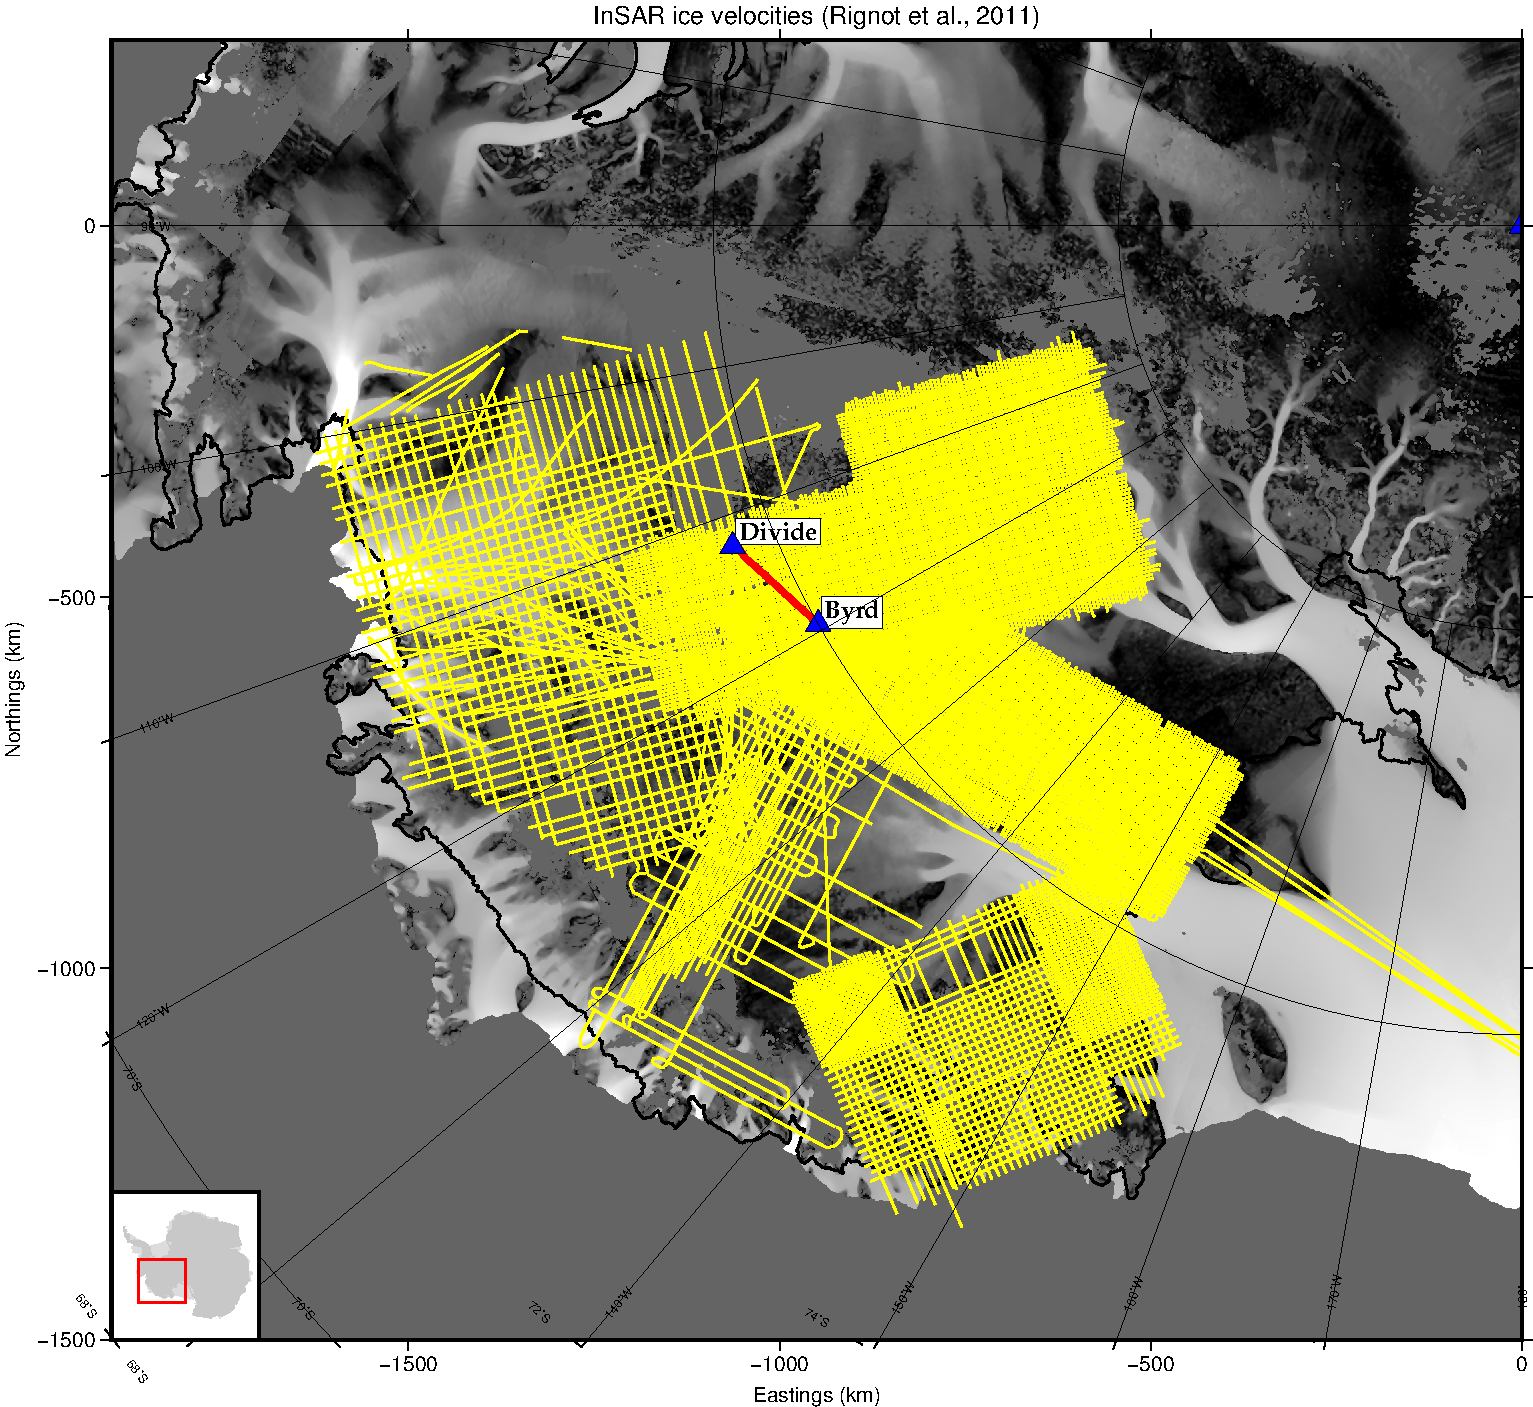
\includegraphics[scale=0.5]{../analysis/figures/WAIS_vel_gray_final}}
%\captionsetup{width=.9\textwidth}
\caption{Map of central West Antarctic with available airborne geophysical radar surveys (yellow lines) and  WAIS Divide and Byrd ice core locations (blue triangles) overlain. Gray shading is surface velocity \citep{rignot2011}. The red line denotes the flight line along which the reflectors in this study were observed. }
\end{figure}



In this study, we consider TWTT of four reflectors spanning the ice thickness in the region of central West Antarctica (Figure~\ref{fig:layergram}). These reflectors have been tracked extensively using Halliburton's Landmark seismic interpretation software and can be tied to both the Byrd and WAIS Divide ice cores for dating. %Determining the depth of the reflectors, $D_r$, may be affected by several sources of uncertainty, including uncertainty in the firn depth, the velocity of the radar pulse in ice, and the pulse-limited precision of radar observations.

\begin{figure}[h]\label{fig:layergram}
\centering
\makebox[\textwidth][c]{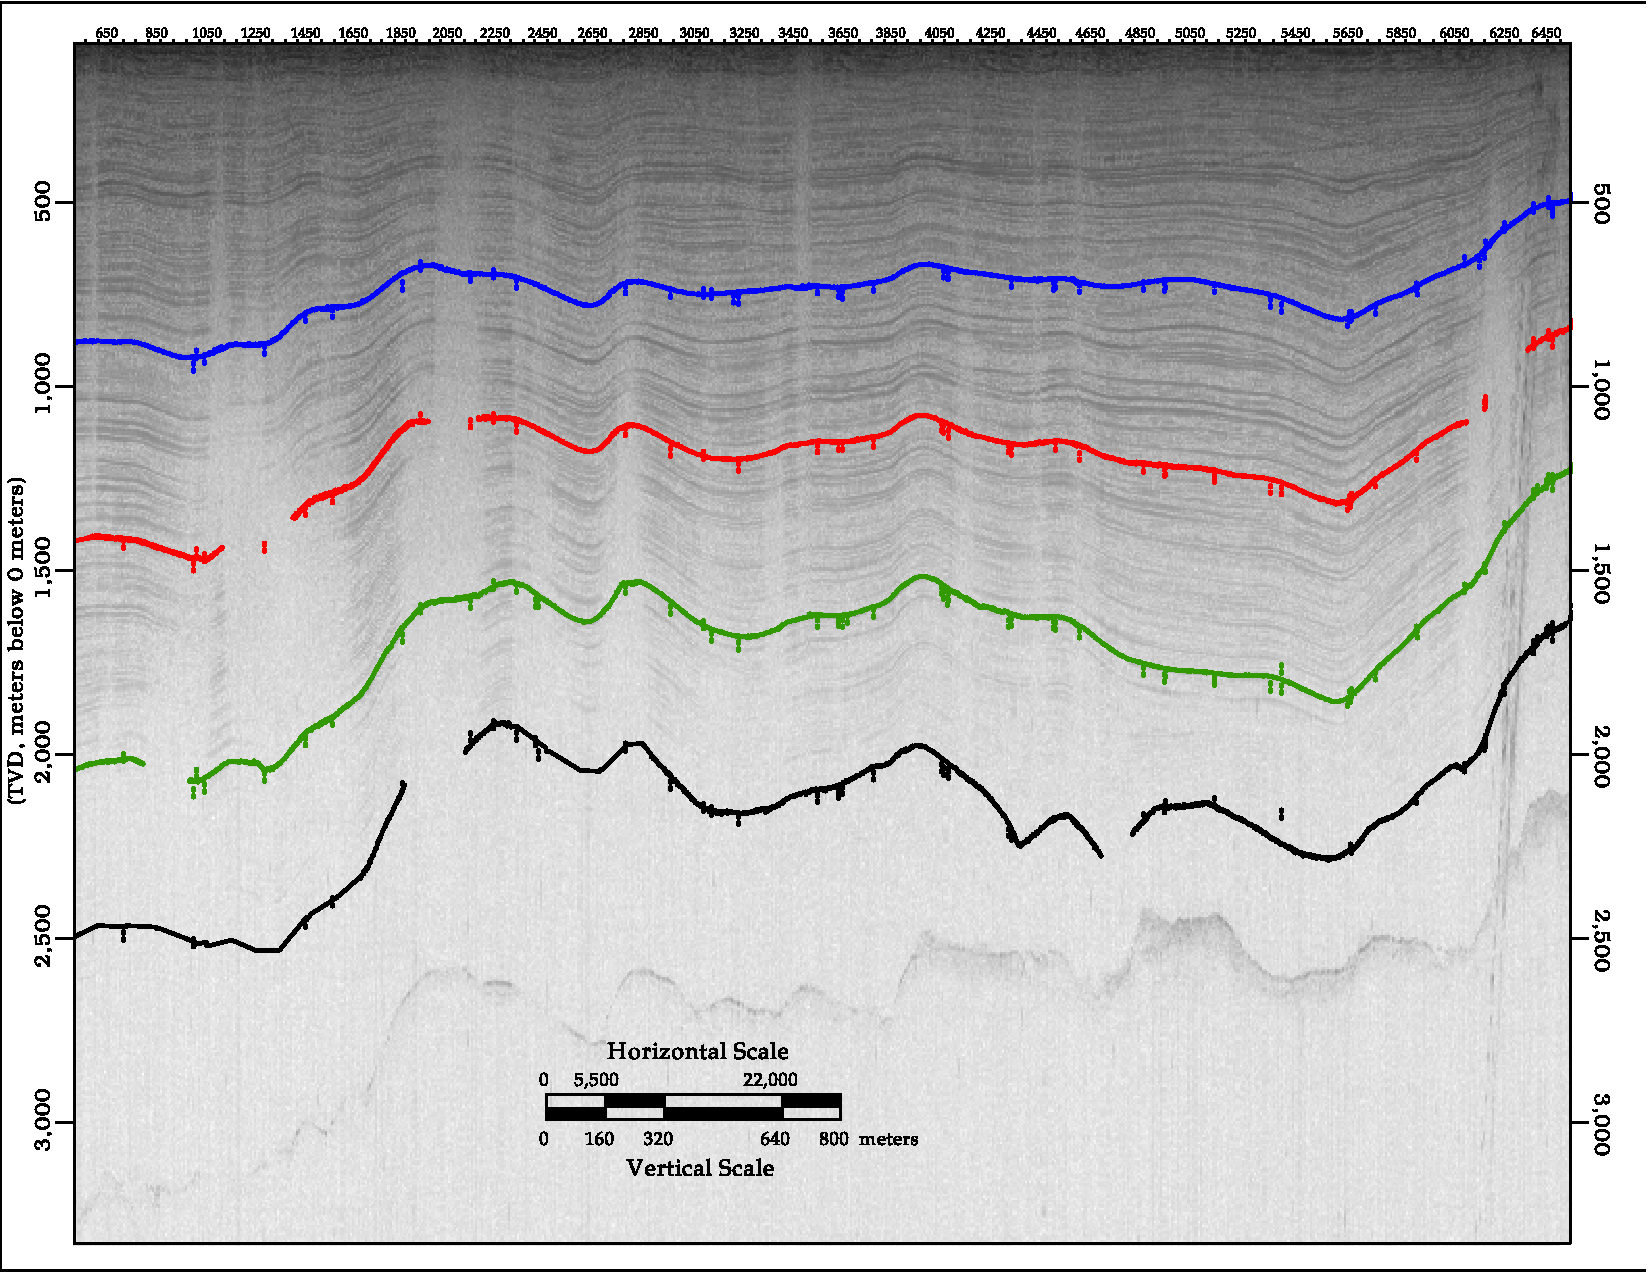
\includegraphics[scale=0.6]{figures/radargram-4layers-paper}}
%\captionsetup{width=.9\textwidth}
\caption{Radargram showing reflectors of interest near the Byrd ice core along flight line ICP6/MKB2l/F14T01a observed using the HiCARS2 radar system. Short vertical hatches along tracked reflectors show intersections with crosslines.}
\end{figure}


To estimate TWTT associated reflector depths, $TWTT_{m,r}(D_r)$, we begin with a simple relation relating different velocities of the radar signal in air and in ice. We incorporate several known sources of uncertainty, including: 1) variations in the signal velocity in ice due to ice temperature and fabric ($v_{ice}$), 2) vertical precision limitations of range detection ($\epsilon_{prec}$), and 3) measurement errors in the density profile needed to account for the changing signal velocity in the firn ($d_{firn}$):

\begin{equation}\label{deptheqn}
%D_r= \frac{1}{2}[(TWTT_r + \epsilon_{prec,r}) - (TWTT_{surf} + \epsilon_{prec,surf})] \cdot v_{ice} + d_{firn}\\
TWTT_{m,r}(D_r) + \epsilon_{prec,r} = 2 \frac{D_r - d_{firn}}{v_{ice}} + (TWTT_{surf} + \epsilon_{prec,surf})
\end{equation}

The complexity of local ice properties affecting the velocity at any location and depth make it difficult to know the true velocity. Empirical evidence suggests a range of expected velocities and we conservatively assume they are uniformly distributed such that: $p(v_{ice}) ~\sim U[168,169.5]\,m/{\mu}s$ \citep{fujita2000}. In lieu of detailed observations of ice properties with depth, we assume the value of $v_{ice}$ is a constant throughout the ice column and apply it systematically to all reflector depths.

The radar pulse width determines vertical precision \citep{millar1982}. We assume a finite pulse width, meaning an infinitesimally thin layer of ice will appear in the survey to have a finite width. This can lead to errors in tracing reflectors, as the reflected energy from a finite depth will include ice with a range of ages. To account for this, we include uncertainty due to range precision error, $\epsilon_{prec}$, of 14 ns \citep{cavitte2016}. We assume this error is normal such that $p(\epsilon_{prec}) = N(0,14)\,ns$. Values of $\epsilon_{prec}$ are sampled for each reflector independently.

Finally, a firn layer with variable density exists in the upper part of the ice sheet. The velocity of the radar signal is faster than in solid ice. To correct for the underestimation of ice depth if the firn layer is not considered, we estimate the difference between the ice thickness with and without the firn layer present ($d_{firn}$). Based on the density profile and firn thickness ($\sim$ 65 m) at the Byrd ice core site \citep{gow1970}, we estimate the prior on $d_{firn}$ to be $p(d_{firn})\sim$ U[6, 36]\,m. 

*******This assumes the firn correction is less than the firn depth itself because we expect velocity in firn will vary from that in glacial ice by only a few percent \citep{robin1975}.  The firn correction is systematically applied to all englacial reflectors of interest in this study because they are alldeeper than the measured firn layer.%Errors in density, $\rho(z)$, are available for the WAIS Divide measurements. These are assumed gaussian, randomly sampled, and the firn correction is computed using the \citet{dowdeswell2004} relation:

%\begin{equation}
%z_f = \frac{K}{n^{'}_{i}}\int{(\rho_{i} - \rho(z)) dz}
%\end{equation}
%where K is 0.85 m$^{3}$ Mg$^{-1}$ \citep{robin1969}, $n^{'}_{i}$ is the refractive index of ice ($n^{'}_{i}$=1.78), $\rho_{i}$ is the density of ice ($\rho_{i}$=0.917 Mg m$^{-3}$) and $\rho(z)$ is the density of ice at depth \textit{z} with units Mg m$^{-3}$.

The TWTT from the observing aircraft to the surface of the ice sheet is known from interpretation of the surface reflector, $TWTT_{surf}$. The computed depth of each reflector is relative to this surface reflector. Just as each reflector may have TWTT precision errors independent of the others, errors in the distance between the surface and the acquisition aircraft are systematic across all observed reflectors in the ice column. Therefore, a randomly sampled precision error, $\epsilon_{prec,surf}$, is also applied to $TWTT_{surf}$ which flattened to 250 ns during data processing. 







